\documentclass{article}

\usepackage[margin=1in]{geometry}
\usepackage{microtype}
\usepackage{setspace}
\usepackage{booktabs}
\usepackage{graphicx}
\usepackage{caption}
\usepackage{pdflscape}
\usepackage{float}
\usepackage{natbib}
\usepackage{amsmath}
\usepackage{enumitem}
\usepackage[hidelinks]{hyperref}
\usepackage[all]{nowidow}

\captionsetup{font=small,labelfont=bf}
\setlength{\parskip}{0pt}
\doublespacing
\AtBeginDocument{\large}

\newcommand{\ConfidenceLevel}{95}
\newcommand{\ControlMean}{6.78}
\newcommand{\ParticipantTtwoMean}{9.25}
\newcommand{\ParticipantTthreeMean}{7.90}
\newcommand{\ControlN}{114}
\newcommand{\ParticipantTtwoN}{105}
\newcommand{\ParticipantTthreeN}{71}
\newcommand{\RecruitmentN}{568}
\newcommand{\ParticipantTtwoFullN}{124}
\newcommand{\ParticipantTthreeFullN}{93}
\newcommand{\ControlFullN}{150}
\newcommand{\MainDifference}{1.12}
\newcommand{\MainLow}{-0.68}
\newcommand{\MainHigh}{2.92}
\newcommand{\MainP}{$= .215$}
\newcommand{\MainRatio}{1.17}
\newcommand{\MainRatioLow}{0.92}
\newcommand{\MainRatioHigh}{1.48}
\newcommand{\MainPercent}{16.5}
\newcommand{\AdjustedDifference}{0.97}
\newcommand{\AdjustedLow}{-0.83}
\newcommand{\AdjustedHigh}{2.77}
\newcommand{\AdjustedN}{174}
\newcommand{\PairedDifference}{-0.87}
\newcommand{\PairedLow}{-3.44}
\newcommand{\PairedHigh}{1.70}
\newcommand{\SecondaryDifference}{2.47}
\newcommand{\SecondaryLow}{0.20}
\newcommand{\SecondaryHigh}{4.74}
\newcommand{\BalanceDifference}{-0.01}
\newcommand{\BalanceLow}{-0.14}
\newcommand{\BalanceHigh}{0.12}
\newcommand{\BalanceP}{$= .871$}
\newcommand{\PairedBalanceDifference}{-0.20}
\newcommand{\PairedBalanceLow}{-0.42}
\newcommand{\PairedBalanceHigh}{0.02}
\newcommand{\PairedBalanceP}{$= .068$}
\newcommand{\AbsoluteDifference}{-0.04}
\newcommand{\AbsoluteLow}{-0.15}
\newcommand{\AbsoluteHigh}{0.06}
\newcommand{\PairedAbsoluteDifference}{-0.19}
\newcommand{\PairedAbsoluteLow}{-0.33}
\newcommand{\PairedAbsoluteHigh}{-0.05}
\newcommand{\CoderAgreement}{92.0}
\newcommand{\CoderAlpha}{0.79}
\newcommand{\UnresolvedSlots}{88}


\title{How Can You Think That?\\Deliberation and the Learning of Opposing Arguments}
\author{Gaurav Sood \and Robert C. Luskin \and James S. Fishkin}
\date{September 2026}

\begin{document}
\maketitle

\begin{abstract}
Deliberation is commonly thought to increase people's awareness of both supporting and
opposing arguments. But who learns, and what can an observational comparison tell us about
that learning? We revisit a Deliberative Poll in Northern Ireland on the future of the school
system. Its questionnaire asked respondents to list reasons that people supporting and opposing
four policies might offer. One month after the event, participants gave an average of
\ParticipantTthreeMean{} coded reasons and contemporaneous controls gave \ControlMean{}.
The difference is \MainDifference{} reasons (\ConfidenceLevel\% confidence interval: \MainLow{} to
\MainHigh{}). Adjustment for age, sex, religious community, and degree status yields a similar
estimate, but the intervals are wide. Participation was self-selected, and the open-ended
measure was not administered at the initial recruitment interview. The evidence therefore
shows a positive but imprecise association, not an identified causal effect of deliberation.
Participants did not differ detectably from controls in directional balance. Among the smaller
complete-case panel, however, supporting and opposing repertoires became more balanced between
the end of the event and the follow-up; coder-specific estimates are weaker. Even in this
difficult setting, respondents could state reasons on both sides. Whether deliberation caused
them to learn those reasons remains open.

\medskip
\noindent\textbf{Keywords:} deliberation, political knowledge, opposing arguments,
\\Northern Ireland, Deliberative Polling
\end{abstract}

\newpage
\section{Introduction}

In their everyday lives, many people have little idea how others holding policy preferences
very different from theirs could do so \citep{mutz2002cross}. The least attentive may not even
recognize the existence of opposing opinions. Others may recognize their existence but never
trouble to wonder how they could be held. Yet others may recognize their existence but be at a
loss to explain them. And yet others may recognize them and attribute them to ignorance,
stupidity, prejudice, or naked self-interest.

For that matter, some people---again, the least attentive---may have no conscious reason for
their own policy preference. Some indeed have no real preference, and report ``non-attitudes''
in response to survey questions \citep{converse1964nature,converse1970attitudes}. Others may have a preference
and one or more conscious reasons for it. They may even recognize, without accepting, a few
more. But many recognize only a few of the plausible reasons for their own views, and of course
hold still fewer.

Deliberation may to some degree remedy all this. Deliberation, as the term is most commonly
employed, is discussion, but not just any discussion. It is balanced, exposing its participants
to competing arguments. It is informative, involving an exchange of information broadly
construed. It is earnest, in the participants' considering and weighing each other's views while
leaving open the possibility of changing their own. And it is civil.

The process should inject its participants' everyday political reality with a good dose of
additional cognition. It should increase their recognition and internalization of the possible
reasons for their own existing preferences, enriching and possibly nuancing them, if not
necessarily altering their broad thrust. That in itself can be normatively valuable insofar as
it moves them closer, at least as a matter of degree or nuance, toward their considered or
full-information views \citep{tocqueville1969democracy,fishkin1991democracy,
dahl1989democracy,arendt1968truth}.

More distinctively, however, deliberation should increase participants' awareness of the
possible reasons for opposing preferences. That may be still more valuable, enriching and
possibly nuancing their existing preferences---and sometimes altering their broad thrust when
a change would make them more considered. That is one possible benefit. The other is that
participants who learn more of the other side's reasons may regard them with greater respect,
understanding better how others could legitimately, if mistakenly, disagree.

But who learns how many supporting and opposing arguments? How is that learning conditioned
by what participants bring to the process? And what can the available comparison groups
actually establish? We examine these questions using data from a Deliberative Poll on the
future of the school system in the Omagh District Council area of Northern Ireland. The design
does not warrant treating participant--control differences as effects of deliberation:
respondents selected themselves into the event, and the study did not measure the open-ended
outcome at recruitment. We therefore distinguish what the data describe from the causal account
that motivated their collection.

\section{Arguments}

Let us begin by underscoring some conceptual distinctions. First, we are primarily concerned
with the learning of reasons, not the persuasion or attitude change that may sometimes ensue.
To cognize arguments is not necessarily to accept them, much less to accept enough of them to
change one's views. Participants in a deliberation may reject many, most, or all of the
arguments they learn. What we examine is movement from ``How could you think that?'' to ``I
can see how you could think that'' (and from ``Why do I think that?'' to ``That's why I think
that''). In most cases, ``I can see how you could think that'' would in fuller form be followed
by ``although I still disagree.''

It is important to keep in mind that the ``sides'' here are sides of a policy debate, not
sectarian groups. The question is the learning of arguments, especially those favoring the
other side of the debate. This is not to say that identification with a sectarian group cannot
affect learning. Where relations between groups are hostile, intergroup animus may lead some
people to ignore arguments made by the opposing group, regardless of their content. If the
issue touches the sectarian cleavage, people may be especially unlikely to learn arguments
about sharing resources or working together.

Prior work calls the relevant reasons people can give for their own and opposing opinions an
argument repertoire \citep{cappella2002argument}. Some explicit terminology and notation
make the argument clearer. For simplicity, assume a binary choice between policy options $A$
and $B$, where $B$ may simply mean not-$A$. An argument may be pro- or anti-$A$. Denote the
numbers of pro- and anti-$A$ arguments in long-term memory by $n_p$ and $n_a$, their combined
number by $n_c=n_p+n_a$, and their directional balance by

\begin{equation}
b_A=\frac{n_p-n_a}{n_p+n_a}.
\end{equation}

If $n_a=0$, then $b_A=1$; if $n_p=0$, then $b_A=-1$; and if $n_p=n_a$, then
$b_A=0$. Absolute imbalance is $|b_A|$. These quantities are implicitly indexed by person,
topic, and measurement wave.

An argument's being ``supporting'' or ``opposing'' depends on the agreement or disagreement of
its thrust with the individual's own position. Because we examine change over time, the
relevant position is the initial one. Supporting arguments buttress that position; opposing
arguments undermine it. Let $s$ and $o$ denote those counts. The total measured repertoire and
its balance are

\begin{equation}
c=s+o, \qquad b=\frac{s-o}{s+o}, \qquad a=|b|.
\end{equation}

Directional balance ranges from $-1$, when every reason is opposing, to $1$, when every reason
is supporting. Absolute imbalance $a$ ranges from zero to one. Balance is undefined when
$s+o=0$; such respondent-waves do not enter analyses of $b$ or $a$. For someone who initially
favors a policy, pro-policy reasons are supporting and anti-policy reasons opposing. The labels
reverse for someone who initially opposes it.

Parallel variables can characterize the arguments aired in the deliberation. Some may not
reside in the head of any participant at the outset; most are presumably cognized by some but
by no means all. Denote the available pro- and anti-$A$ arguments by $N_p$ and $N_a$. These are
outside-the-head entities residing in communications, not necessarily represented in every
participant's belief system.

\subsection{Deliberation and the learning of arguments}

At any moment, the number of pro-$A$ arguments a person knows is a function of historical
exposure to such arguments and historical incentives to absorb them. Illustratively, with no
commitment to a particular functional form,

\begin{equation}
n_p=f(\alpha_0+\alpha_1N_p+\alpha_2I_p), \qquad
n_a=f(\alpha_0+\alpha_1N_a+\alpha_2I_a).
\end{equation}

The parameters need not differ for pro- and anti-$A$ arguments. The point is to distinguish
exposure from attention and retention, a distinction long emphasized in work on information
seeking and political communication \citep{atkin1973instrumental,chaffee1972interpersonal,
chaffee1973individual}.

\paragraph{H1: Deliberation increases the total number of cognized arguments.}
Deliberation should promote the learning of ``new'' arguments---perhaps previously
encountered, but not previously cognized---both pro and con. It adds exposure and incentives:
thinking about arguments is part of the task. Thus deliberation should increase both $n_p$ and
$n_a$, just as Deliberative Polls have often increased factual knowledge
\citep{hansen2004deliberative,luskin2009learning}.

\paragraph{H2: In everyday life, cognized supporting arguments should outnumber cognized
opposing arguments.}
People generally encounter and retain more attitudinally congenial than uncongenial
considerations \citep{mutz2002cross,baron1998judgment}. Adjacent research finds similar
asymmetries for political facts and their interpretation
\citep{dellicarpini1991stability,dellicarpini1997what,bartels2002beyond,
shapiro2008facts,jerit2012partisan,
gaines2007same}.

Part of this story is social exposure. People often live among others sharing their political
orientations \citep{bishop2009big,abrams2012big,cho2013voter,mcdonald2011migration}. They also select associates with similar
views \citep{verbrugge1977structure,verbrugge1983research,huckfeldt1995citizens,
mutz2001facilitating,mackuen1990speaking,bennett2000political}. When they nevertheless interact with people holding
opposing views, an interest in avoiding discord may keep disagreement off the table.

People also seek and select information that confirms existing views. The tendency applies to
policy-relevant information and media choice \citep{iyengar2008selective,
garrett2009politically,iyengar2009red,
stroud2008media,sunstein2001republic}. Once exposed, people process information less as neutral
observers than as interested partisans \citep{chang2003party,lord1979biased}. Exposure,
attention, and retention may therefore all favor supporting reasons.

\paragraph{H3: Deliberation narrows the everyday imbalance between supporting and opposing
arguments.}
Deliberation should increase the total repertoire and may narrow its imbalance. The two claims
are distinct. It airs arguments on both sides, more or less equally, but the newly encountered
arguments need only be less imbalanced than the old repertoire. Suppose deliberation adds
$\Delta s$ supporting and $\Delta o$ opposing reasons. Then

\begin{equation}
b'-b=
\frac{2(o\Delta s-s\Delta o)}
{(s+o)(s+o+\Delta s+\Delta o)}.
\end{equation}

When the initial repertoire favors supporting reasons and all relevant quantities are positive,
imbalance narrows if $\Delta s/\Delta o<s/o$: the new reasons need not be evenly divided, only
less one-sided than the old repertoire. Total growth alone therefore says nothing about whether
someone has become better able to articulate the opposing side.

Deliberation may supply just such a stream. It airs reasons on both sides and gives opposing
reasons faces. A reason offered by a person one now knows is harder to ignore. Attention and
retention may remain selective, but the new exposure and incentives should be less one-sided
than those of everyday political life.

\subsection{Conditioning factors}

Other variables may condition these expectations. Anything that produces a scant initial store
of arguments may also depress the number learned. Anything that accentuates the initial
imbalance creates more room for deliberation to level it. And anything that preserves unequal
incentives to absorb supporting and opposing arguments may reduce that leveling.

\paragraph{H4: Policy attachments may dampen the learning of opposing arguments.}
Forced exposure does not eliminate selective attention and retention. People who favor $A$
may be less likely to learn anti-$A$ arguments, while those who oppose $A$ may be less likely to
learn pro-$A$ arguments. Deliberation can therefore increase the total repertoire without
producing symmetric gains or narrowing imbalance.

\paragraph{H5: Intergroup hostility may dampen both learning and the narrowing of imbalance.}
Suppose a population is divided into groups such as Catholics and Protestants. Dislike of the
other group may limit attention to arguments associated with its members. The problem is most
acute when group membership is correlated with position on the issue: members of each group
may then tune out the arguments disproportionately offered by the other. On issues expressly
involving group rights, resources, or contact, intergroup affect may also spill directly into
the policy judgment \citep{altemeyer1996authoritarian,marcus1995malice,kim2011contact}.
Yet these conditions need not all hold. If Catholics and Protestants take
similar positions on an issue, participants can hear both sides from members of both groups.

\paragraph{H6: Deliberation may produce a larger increase among those who already know more.}
Participants arriving with more arguments may learn still more, just as those arriving with
more factual knowledge often acquire more in information-rich settings. Existing knowledge can
provide hooks for organizing new material rather than crowding it out. This expectation sits
against the generally low-information environment of mass politics, in which acquiring and
organizing policy information is costly and uneven
\citep{downs1957economic,iyengar1990shortcuts,gilens2001political}.

\paragraph{H7: Learning, especially of opposing arguments, may be greater in more
attitudinally diverse groups.}
Sociodemographic diversity need not matter except insofar as it predicts policy attitudes. But
encountering people with opposing positions should increase exposure to their reasons. At the
group level, that opportunity is greatest when the group is divided rather than unanimous.

These seven propositions reproduce the theoretical setup that motivated the original study.
The available design, however, does not identify all seven as causal hypotheses. The revised
analysis directly estimates repertoire size and directional balance. Policy attachment,
intergroup hostility, prior knowledge, and group composition remain mechanisms for a design
with baseline repertoire measurement and verified random group assignment. The algebra
organizes the estimands; it is not offered as a new formal model.

\section{The Omagh Deliberative Poll}

The Deliberative Poll took place in Omagh, a district council area in County Tyrone, Northern
Ireland, with nearly 48,000 inhabitants at the time. Omagh had a mixed population of Catholics
and Protestants and primary and post-primary schools representing all the major school types.
Some schools had mainly Catholic pupils, some mainly Protestant pupils, and a few a more even
mix. As in Northern Ireland as a whole, the birthrate and school-age population were declining,
forcing schools to consider greater coordination or consolidation \citep{deni2007schools}.

The setting was a classic deeply divided society with a still-recent history of violent strife.
The Protestant--Catholic divide was reinforced by residential segregation, divided public
housing, segregated schooling, endogamy, and historically distinct employment patterns
\citep{boyle1994northern,ohara2004self,cohen2007stop,pogatchnik2008despite}. From the
standpoint of those skeptical of mass deliberation across deep divisions, bringing randomly
sampled parents together to discuss schools was itself consequential. At the same time,
Catholics and Protestants did not divide neatly on every policy considered here, so sectional
hostility need not translate directly into refusal to learn a policy argument. A companion
account examines this event and deliberation across the community divide in detail
\citep{luskin2014deep}.

The event followed the standard Deliberative Poll design
\citep{fishkin1991democracy,luskin2002better,luskin2002considered,fishkin2009people}. A random sample of parents of school-aged
children was interviewed at recruitment and invited to a long day of deliberation. Of the
\RecruitmentN{} initial interviewees, \ParticipantTtwoFullN{} took part. Participants received
balanced briefing materials and met in moderated small groups, alternating with plenary
sessions in which they questioned policy experts and representatives of the different school
types. Participants completed a survey at the end of the event. A separate control group was
interviewed later, together with a subset of participants roughly one month after the event.
The corresponding analytic counts before coding exclusions are \ControlFullN{} controls and
\ParticipantTthreeFullN{} returning participants.

Like other Deliberative Polls, the Omagh event brought a diverse set of people together in an
environment intended to support a respectful airing of both similarities and differences. In
expectation, participants encountered common briefing materials and the same plenary program,
while their small-group discussions supplied varying mixes of facts, experiences, and reasons.
Those ingredients motivate the learning hypotheses, but they do not make every participant's
experience uniform.

Nor do Northern Ireland's deep divisions necessarily pose the same obstacle for every policy.
Let $A$ be a proposal involving religious mixing. Hostility toward the other community may be
one reason to oppose $A$, and an opponent may initially possess many more anti-$A$ than
pro-$A$ reasons. During deliberation, that person could ignore pro-$A$ arguments associated
with the other community. But the process could also make those arguments more difficult to
ignore, especially when similar arguments come from members of the person's own community.
The direction of the resulting change is therefore an empirical question, not something the
social cleavage settles by itself.

This design contains both an experiment and an observational comparison, and they should not
be conflated. Participants were reportedly assigned to small discussion groups at random. If
that assignment is verified, contrasts among group compositions may support causal claims
about those compositions. Attendance at the event was not randomly assigned: invitees chose
whether to attend. The participant--control contrast can therefore reflect pre-existing
differences, event participation, briefing exposure, measurement timing, or any combination of
them. The original setup supplies the mechanisms and expectations; the revised empirical
sections state more narrowly what these comparisons can establish.

\section{Measurement}

\subsection{Open-ended questions}

The post-event and follow-up surveys contained paired open-ended questions about four school
policies: all-ability schools, balanced religious enrolment, classroom collaboration between
schools of different religious composition, and combining primary with post-primary pupils.
For each policy, respondents could list up to five reasons that strong supporters might offer
and up to five reasons that strong opponents might offer. Closed-ended policy questions allow
us to classify each elicited reason as supporting or opposing the respondent's initial position.

For all-ability schools, respondents first rated the option of ``having a system of all-ability
schools, all providing the same wide curriculum.'' They were then asked for up to five reasons
that people who strongly supported the proposal would give and up to five reasons that people
who strongly opposed it would give.

For combining schools, respondents rated the option of schools combining primary and
post-primary pupils---for example, ages 7--14. The follow-ups again asked separately for the
reasons strong supporters and strong opponents would give.

For collaboration across schools, respondents rated whether, when schools of different
religious composition entered partnerships, children from both schools should at least
sometimes be taught in the same classroom. The paired open-ended questions asked for the
reasons of those who strongly agreed and those who strongly disagreed.

For balanced enrolment, the closed-ended item ran from the view that children should attend
school only with children of their own religion to the view that they should attend schools
with a balanced enrolment of Protestant and Catholic pupils. Respondents then listed reasons
for each endpoint. These prompts asked respondents to reproduce arguments that people on each
side might offer; they did not ask respondents to endorse those arguments.

Two coders, blind to the hypotheses, classified each response by its substance. A third coder
was assigned to adjudicate disagreements. The source file stores a label set from each coder,
because one response could contain more than one reason. The coding pipeline parses those
sets explicitly. It regards reordered sets as agreements, uses the adjudicator when the first
two coders disagree, and leaves a disagreement unresolved when no adjudication is present.
Normalized exact agreement is \CoderAgreement\%, and nominal Krippendorff's $\alpha$ is
\CoderAlpha{}. There are \UnresolvedSlots{} unresolved response slots. These reliability
statistics describe the reproducibility of the coding decisions; they do not validate the
construct itself \citep{krippendorff1980content,krippendorff1986information,
krippendorff2004content}.

The main count gives credit to an answer if it offers at least one reason for a policy view.
Answers coded as nonsense, missing, or too vague do not count. For three questions, code 3 means
the answer calls people with that view prejudiced or ignorant. We leave that code out of the
main count and include it in a separate check. Another valid code in the same answer still
counts. We also check results using every valid code and each original coder's labels. If the
coders disagree and no third coder settles it, we leave that respondent's main count missing
for that survey; the single-coder checks still include the respondent.

Directional outcomes sum supporting and opposing reasons across policies for which the
respondent has a nonneutral initial position. We calculate $b$ and $|b|$ only when both sums
are observed and their combined total is positive. This complete-case rule keeps an unresolved
slot from being silently treated as no reason. Because that rule reduces the paired sample, we
also report the balance estimates separately for each original coder.

\subsection{Other measures}

The questionnaires also measured factual knowledge of the school system, policy attitudes,
religious affiliation, education, age, and sex. They included feeling ratings toward Catholics
and Protestants and trait ratings of whether members of each community were trustworthy and
open to reason. The original study used these variables to motivate analyses of selection,
intercommunity affect, prior knowledge, and group composition.

For the revised primary comparison, age is measured in years; sex is represented by an
indicator for women; religious community distinguishes Catholic and Protestant respondents;
and degree status records whether the respondent reports a bachelor's degree or higher. The
\hyperref[sec:supplement]{Supporting Information} shows these variables across recruitment, attendance, return, and
control samples. The primary adjustment uses them to describe measured composition, not to
claim that selection has been eliminated.

The original group-level argument used the mean factual knowledge of the other participants in
the discussion group and an index of attitudinal heterogeneity across the four policy items.
The latter follows the variance--covariance construction described by
\citet{anderson2003introduction}.
Those quantities remain conceptually relevant to H6 and H7. We do not treat their associations
with post-event responses as causal here because the documentation available in the repository
does not independently verify the small-group randomization or support the original multilevel
specification. They are therefore mechanisms for future analysis rather than parts of the
primary claim.

\subsection{Analytic comparisons}

The primary estimand is the respondent-level mean difference in the total number of coded
reasons between returning participants and contemporaneously interviewed controls. We report
the raw difference and an ordinary least squares adjustment for age, sex, religious community,
and degree status. The adjustment addresses measured composition only. It does not turn the
comparison into an experiment.

Two comparisons are secondary. First, we compare each returning participant's end-of-event
and follow-up responses. The paired change describes retention or decay among returnees, but
it also combines changes in effort, survey context, and mode. Second, we compare all end-of-
event participants with later controls. That contrast has a larger sample but is not
contemporaneous and includes any learning from the briefing materials before the end-of-event
survey.

These comparisons face several distinct threats. Attendance was voluntary: of the people who
completed the recruitment interview and were invited, most did not attend. Some participants
then failed to return the later questionnaire. Sampling variation, selection into attendance,
and attrition can each alter the composition of the samples. The available covariates reveal
some of that composition but cannot establish comparability on motivation, political interest,
verbal fluency, or willingness to complete open-ended questions. Spillover is also possible if
members of the later control sample encountered discussion or materials connected with the
event. Finally, a Deliberative Poll is a collection of parallel small-group experiences rather
than one perfectly uniform treatment.

The original paper described the T2--control and T3--control contrasts as treatment effects.
That wording was too strong. The event invitation did not randomize attendance, and the
open-ended outcome was not measured at recruitment. The revised analysis calls these sample
differences and reserves causal language for a design that identifies the relevant contrast.
For the same reason, we do not repeat the original mediation analysis. A formal mediation
estimator \citep{imai2010general} cannot rescue a treatment effect that the research design
does not identify.

For the directional outcomes, we estimate the same contemporaneous T3 contrast and paired
T2--T3 change. The supporting and opposing totals show which side changes. Directional balance
shows the net tilt toward a respondent's initial position, while absolute imbalance asks only
how far the repertoire lies from parity.

The unit of analysis is the respondent. Participants may share shocks induced by their
moderated discussion group, while controls were not grouped. Confidence intervals therefore
use CR2 standard errors, clustering participants by their observed discussion group and
treating controls as singleton clusters, with Satterthwaite degrees of freedom. This
adjustment addresses dependence; it does not repair the observational comparison. The analysis
is unweighted because the available files do not contain a documented sampling weight for
these comparisons.

\section{Results}

\subsection{Total reasons}

Figure~\ref{fig:means} shows the respondent-level means. Returning participants at follow-up
gave \ParticipantTthreeMean{} coded reasons on average, compared with \ControlMean{} among
controls. The unadjusted difference is \MainDifference{} reasons (\ConfidenceLevel\% confidence interval:
\MainLow{} to \MainHigh{}; $p$ \MainP). The adjusted difference is
\AdjustedDifference{} reasons (\ConfidenceLevel\% confidence interval: \AdjustedLow{} to
\AdjustedHigh{}; complete-case $N=\AdjustedN$). Both estimates are positive, but both
intervals include zero and differences of substantively meaningful size in either direction.
On a multiplicative scale, participants gave \MainPercent\% more reasons than controls
(count ratio \MainRatio{}, \ConfidenceLevel\% confidence interval: \MainRatioLow{} to
\MainRatioHigh{}). The ratio is useful for magnitude; it remains an associational comparison.

\begin{figure}[htbp]
\centering
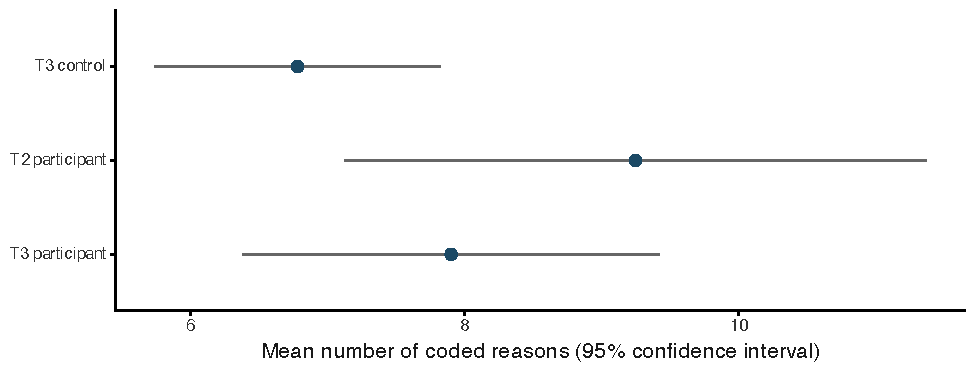
\includegraphics[width=\textwidth]{../figs/mean_reason_counts.pdf}
\caption{Mean number of coded reasons by sample and wave. Points are respondent-level means;
lines are \ConfidenceLevel\% CR2 confidence intervals using participant discussion groups and singleton
control clusters. The primary coding excludes invalid and vague
responses, question-specific answers that give the other side too little credit, and respondent
waves containing an unresolved coder disagreement. The T2 participant and T3 control samples
were not interviewed contemporaneously.}
\label{fig:means}
\end{figure}

The paired estimate is also imprecise. Among returnees with resolved coding at both waves,
the follow-up total changes by \PairedDifference{} reasons relative to the end-of-event total (\ConfidenceLevel\%
confidence interval: \PairedLow{} to \PairedHigh{}). The noncontemporaneous end-of-event
participant difference is larger: \SecondaryDifference{} reasons (\ConfidenceLevel\% confidence interval:
\SecondaryLow{} to \SecondaryHigh{}). That pattern is consistent with short-run exposure or
effort followed by decay, but the design cannot distinguish that account from selection and
measurement differences.

\begin{table}[htbp]
\centering
\caption{Primary and secondary respondent-level comparisons}

\begin{tabular}{lllrr}
\toprule
Panel & Sample or contrast & Quantity & Estimate [95\% CI] & $N$\\
\midrule
Means & T3 control & Mean & 6.78 [5.73, 7.83] & 114\\
Means & T2 participant & Mean & 9.25 [7.13, 11.37] & 105\\
Means & T3 participant & Mean & 7.90 [6.38, 9.42] & 71\\
Comparisons & T3 participant minus T3 control, unadjusted & Difference & 1.12 [-0.68, 2.92] & 185\\
Comparisons & T3 participant minus T3 control, adjusted & Difference & 0.97 [-0.83, 2.77] & 174\\
Comparisons & Participant change, T3 minus T2 & Difference & -0.87 [-3.44, 1.70] & 62\\
Comparisons & T2 participant minus T3 control & Difference & 2.47 [0.20, 4.74] & 219\\
Comparisons & T3 participant divided by T3 control & Mean ratio & 1.17 [0.92, 1.48] & 185\\
\bottomrule
\end{tabular}

\begin{minipage}{\textwidth}
\smallskip\footnotesize
\textit{Note:} Differences are in coded reasons. Intervals use CR2 standard errors with
Satterthwaite degrees of freedom. Participant observations are clustered by discussion group;
controls are singleton clusters. The adjusted T3
comparison includes age, sex, religious community, and degree status. The paired row compares
the same returning participants. The last row compares samples interviewed at different times.
\end{minipage}
\end{table}

\subsection{Supporting, opposing, and balanced repertoires}

Table~\ref{tab:directional} separates repertoire size from direction. At T3, participants gave
slightly more supporting and opposing reasons than controls. But their directional balance
differs by only \BalanceDifference{} (\ConfidenceLevel\% confidence interval: \BalanceLow{} to
\BalanceHigh{}; $p$ \BalanceP), and their absolute imbalance by \AbsoluteDifference{}
(\ConfidenceLevel\% confidence interval: \AbsoluteLow{} to \AbsoluteHigh{}). The
participant--control association in total repertoire is therefore not concentrated in a clear
shift toward the opposing side.

The paired comparison is different. Among returnees with complete primary coding and a
positive repertoire at both waves, directional balance changes by
\PairedBalanceDifference{} (\ConfidenceLevel\% confidence interval:
\PairedBalanceLow{} to \PairedBalanceHigh{}; $p$ \PairedBalanceP), while absolute imbalance
changes by \PairedAbsoluteDifference{} (\ConfidenceLevel\% confidence interval:
\PairedAbsoluteLow{} to \PairedAbsoluteHigh{}). The interval for signed balance includes zero,
while the decline in absolute imbalance indicates movement toward parity in this complete-case panel. Most of the movement comes from fewer supporting reasons rather than more
opposing reasons, so it is evidence of narrowing, not evidence that respondents accumulated
opposing reasons during the month.

\begin{table}[htbp]
\centering
\small
\caption{Supporting and opposing argument repertoires}
\label{tab:directional}
\resizebox{\textwidth}{!}{%

\begin{tabular}{lrrrrrr}
\toprule
Outcome & T3 control & T3 participant & T3 difference [95\% CI] & $N$ (T3) & Paired change [95\% CI] & $N$ (paired)\\
\midrule
Supporting reasons & 3.40 & 3.71 & 0.32 [-0.59, 1.23] & 211 & -1.10 [-2.11, -0.08] & 72\\
Opposing reasons & 2.38 & 2.51 & 0.13 [-0.47, 0.74] & 226 & -0.35 [-1.16, 0.46] & 82\\
Directional balance ($b$) & 0.23 & 0.22 & -0.01 [-0.14, 0.12] & 176 & -0.22 [-0.42, -0.02] & 51\\
Absolute imbalance ($|b|$) & 0.37 & 0.33 & -0.04 [-0.15, 0.06] & 176 & -0.20 [-0.33, -0.08] & 51\\
\bottomrule
\end{tabular}

}
\begin{minipage}{\textwidth}
\smallskip\footnotesize
\textit{Note:} Supporting and opposing are defined relative to each respondent's initial
policy position. Counts sum reasons across classifiable policies. Directional balance is
$b=(s-o)/(s+o)$, and absolute imbalance is $|b|$; both are undefined when $s+o=0$.
Differences use CR2 standard errors with Satterthwaite degrees of freedom. T3 differences are
participant minus control; paired changes are T3 minus T2 among returning participants. Sample
sizes vary because unresolved coding, neutral positions, and zero repertoires affect the four
outcomes differently.
\end{minipage}
\end{table}

\begin{figure}[htbp]
\centering
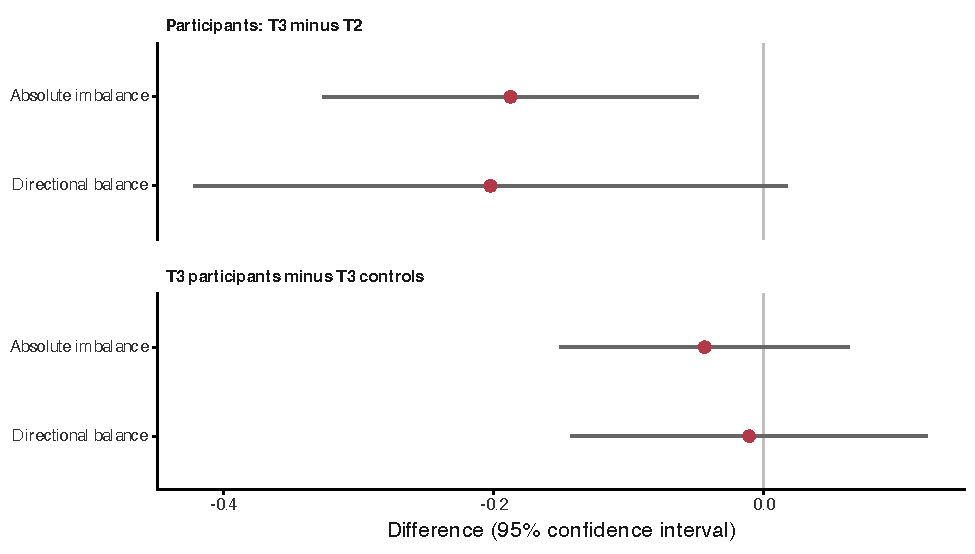
\includegraphics[width=\textwidth]{../figs/argument_balance.pdf}
\caption{Changes in directional balance and absolute imbalance. Points show the T3
participant--control difference and the paired T3--T2 change; lines are \ConfidenceLevel\%
CR2 confidence intervals. Zero denotes no difference or change. Supporting reasons raise
$b$ and opposing reasons lower it; smaller $|b|$ means a more even repertoire.}
\label{fig:balance}
\end{figure}

\subsection{Sensitivity to coding choices}

The inclusive count, the count of coded mentions, and the two coder-specific totals all yield
positive T3 participant--control differences. Their intervals overlap the primary interval and
generally include zero. The coder-specific estimates use the full contemporaneous sample and
show that dropping respondent waves with unresolved adjudication reduces precision without
creating the direction of the result. These sensitivity intervals use the same partially clustered
CR2 procedure as the primary estimate. The paired balance result is more sensitive: both
coder-specific changes point toward greater balance, but they are smaller than the primary
complete-case estimate and their \ConfidenceLevel\% intervals include zero.

\section{What the evidence establishes}

The strongest result is descriptive. Returning participants could articulate reasons on both
sides of contentious school-policy debates in a deeply divided setting. They gave somewhat
more valid reasons than contemporaneous controls, but the estimate is imprecise after the
coding rules are enforced. The data do not establish that deliberation caused the difference.

Participation was self-selected, and the open-ended outcome was not measured in the initial
recruitment interview. Covariate
adjustment can compare respondents who look similar on recorded demographics, but it cannot
remove unmeasured interest, motivation, verbal fluency, or willingness to spend a day at the
event. The later control interview also differs from the participant surveys in timing and
experience. These are properties of the design, not statistical inconveniences that a more
elaborate model can solve.

The paired comparison answers a narrower question. It follows the same people from the end of
the event to the later survey, so stable differences among people do not confound the change.
But the end-of-event survey came after briefing materials and the day's proceedings, and the
follow-up took place under a different context. The decline is compatible with forgetting; it
is also compatible with lower effort or a changed response situation. The same qualification
applies to the apparent narrowing of directional imbalance. Because supporting reasons decline
more than opposing reasons, the result need not reflect new understanding of the opposing side.

The measurement analysis adds a caution. A response can contain multiple reasons, coders can
disagree about its labels, and the primary count requires a decision about whether each response
contains a substantive reason. Explicit set parsing, adjudication states, and coder-specific
sensitivities make those decisions visible. The similarity of the sensitivity estimates is
reassuring for total repertoire size, but the directional paired estimate moves materially when
each original coder is used. Coder agreement cannot establish that the count captures every
relevant kind of argument equally well.

\section{Discussion}

The motivating idea remains important. Deliberation may enable movement from ``How could you
think that?'' to ``I can see how you could think that,'' even when disagreement remains. The
Omagh respondents demonstrate that people in a deeply divided society can state arguments on
both sides of policies touching sectional lines. But a capacity demonstrated in a selected
participant sample is not the same as an average causal effect of deliberation.

Earlier research found that people who encounter cross-cutting political networks tend to be
more aware of arguments on the other side, though such networks can also discourage political
participation \citep{mutz2002cross,mutz2002consequences}. Yet those who choose such
exposure may differ in unmeasured ways from those who do not. Everyday discussion may
sometimes overcome imbalance when it is sustained, engaging, and sufficiently broad. A
structured deliberative event is designed to make those conditions less exceptional. The
remaining empirical problem is to separate what the event caused from the characteristics of
the people who attended it.

This study also remains one Deliberative Poll on one topic. Northern Ireland's divisions affect
many features of its mass and elite politics, including what participants bring to a discussion
about schools. That makes Omagh a demanding and substantively important setting, but it does
not by itself reveal whether the same pattern would appear for other issues, populations, or
forms of deliberation.

One conception of considered preferences asks what people would think if they were well
informed, heard competing opinions, and understood the consequences of the alternatives
\citep{fishkin1991democracy,fishkin2009people,dahl1989democracy,arendt1968truth}. Most
people know and have considered relatively little about most policy questions. Deliberative
Polling seeks to provide factual information and an opportunity to encounter competing
reasons. Learning an opposing argument may therefore matter even when it does not change a
policy preference: continued disagreement can become more informed and more intelligible.

A stronger study would measure the open-ended outcome before invitations or briefing
materials, randomize access to the deliberative event among willing respondents, and repeat the
same measurement after the event and at follow-up. It would preserve the actual arguments,
their coder label sets, and all adjudications in a tidy long format. Such a design would
separate selection, immediate learning, and retention. It would also permit a direct test of
whether gains are concentrated among opposing rather than supporting reasons.

For now, the evidence supports a narrow conclusion. Returning participants articulated
somewhat more reasons than controls, and both groups could articulate
opposing reasons. The T3 comparison shows no detectable difference in directional balance.
The paired complete-case estimate moves toward balance, but its sensitivity to coder choice and
its source in declining supporting reasons limit what it establishes. The uncertainty is too
large, and the design too confounded, to attribute these patterns to deliberation. This is not a
null conclusion about deliberation. It is the question the available evidence can answer.

\bibliographystyle{plainnat}
\bibliography{references}

\newgeometry{margin=0.8in}
\singlespacing
\normalsize
\setlength{\parindent}{0pt}
\setlength{\parskip}{6pt}
\appendix
\setcounter{section}{1}
\renewcommand{\thesection}{S}
\setcounter{table}{0}
\renewcommand{\thetable}{S\arabic{table}}
\phantomsection
\label{sec:supplement}
\addcontentsline{toc}{section}{Supporting Information}
\section*{Supporting Information}

The following tables report expanded descriptive and sensitivity results. Estimates use the
primary coding unless a table states otherwise. Confidence intervals use CR2 standard errors
with Satterthwaite degrees of freedom, clustering participants by discussion group and treating
controls as singleton clusters.

\subsection{Sample composition}

\begin{table}[H]
\centering
\caption{Composition of recruitment, participant, returnee, and control samples}

\begin{tabular}{lrrrrr}
\toprule
Sample & $N$ & Age & Women (\%) & Catholic (\%) & Degree (\%)\\
\midrule
T1 nonparticipant & 444 & 40.0 (436) & 69.1 (444) & 72.6 (424) & 18.8 (441)\\
T2 participant & 124 & 40.7 (124) & 75.8 (124) & 65.8 (120) & 19.5 (123)\\
T3 nonreturning participant & 31 & 37.9 (31) & 74.2 (31) & 66.7 (30) & 12.9 (31)\\
T3 returning participant & 93 & 41.6 (93) & 76.3 (93) & 65.6 (90) & 21.7 (92)\\
T3 control & 150 & 40.0 (149) & 72.7 (150) & 73.9 (142) & 18.7 (150)\\
\bottomrule
\end{tabular}

\begin{minipage}{0.95\textwidth}
\smallskip\footnotesize
\textit{Note:} Cells contain a mean or percentage followed by the nonmissing denominator in
parentheses. T1 nonparticipants completed the recruitment interview but did not attend the
event. T3 nonreturning participants attended but did not complete the follow-up. T3 controls
were recruited separately.
\end{minipage}
\end{table}

\clearpage
\begin{landscape}
\subsection{Policy-specific results}

\begin{table}[H]
\centering
\scriptsize
\caption{Mean coded reasons and contrasts by policy and prompt}
\resizebox{\linewidth}{!}{%

\begin{tabular}{llrrrrrr}
\toprule
Policy & Prompt & T2 P & T3 P & T3 C & T2 P $-$ T3 C & T3 P $-$ T3 C & T3 $-$ T2\\
\midrule
All-ability schools & Pro-policy & 1.71 (118) & 1.19 (89) & 1.00 (147) & 0.71 [0.31, 1.12] (265) & 0.19 [-0.11, 0.50] (236) & -0.56 [-1.03, -0.10] (85)\\
All-ability schools & Anti-policy & 1.19 (119) & 0.85 (92) & 0.83 (145) & 0.37 [-0.03, 0.77] (264) & 0.02 [-0.24, 0.28] (237) & -0.43 [-0.91, 0.06] (89)\\
Balanced enrolment & Anti-policy & 1.49 (123) & 1.13 (92) & 0.98 (146) & 0.51 [0.22, 0.79] (269) & 0.15 [-0.13, 0.43] (238) & -0.30 [-0.64, 0.04] (92)\\
Balanced enrolment & Pro-policy & 1.88 (118) & 1.60 (78) & 1.26 (127) & 0.62 [0.19, 1.05] (245) & 0.34 [0.01, 0.67] (205) & -0.20 [-0.61, 0.21] (74)\\
Inclusive classrooms & Pro-policy & 1.37 (124) & 1.10 (92) & 1.01 (147) & 0.36 [0.01, 0.72] (271) & 0.09 [-0.19, 0.37] (239) & -0.30 [-0.69, 0.08] (92)\\
Inclusive classrooms & Anti-policy & 0.64 (121) & 0.49 (93) & 0.57 (150) & 0.07 [-0.18, 0.32] (271) & -0.08 [-0.29, 0.13] (243) & -0.12 [-0.49, 0.25] (90)\\
Combined primary and post-primary schools & Pro-policy & 0.92 (123) & 1.02 (93) & 0.72 (149) & 0.19 [-0.08, 0.47] (272) & 0.30 [0.04, 0.55] (242) & 0.11 [-0.25, 0.47] (92)\\
Combined primary and post-primary schools & Anti-policy & 0.79 (122) & 0.92 (91) & 0.81 (149) & -0.02 [-0.35, 0.31] (271) & 0.12 [-0.15, 0.38] (240) & 0.16 [-0.25, 0.56] (90)\\
\bottomrule
\end{tabular}

}
\begin{minipage}{0.96\linewidth}
\smallskip\footnotesize
\textit{Note:} T2 P and T3 P denote participants at the end of the event and follow-up; T3 C
denotes contemporaneous controls. The first two differences compare distinct samples. T3
minus T2 is a within-returnee change. Contrast cells contain an estimate and 95\% confidence
interval. Prompt labels refer to the policy direction, not to the respondent's own position.
Parentheses contain the sample size for each mean or contrast.
\end{minipage}
\end{table}
\end{landscape}

\subsection{Response-slot order}

\begin{table}[H]
\centering
\caption{Linear probability model for whether a response slot contains a valid reason}

\begin{tabular}{lrrrrrr}
\toprule
Term & Estimate & CR2 SE & CI low & CI high & Rows & Clusters\\
\midrule
T3 participant & 0.076 & 0.036 & 0.002 & 0.149 & 9656 & 170\\
Response-slot order & -0.130 & 0.006 & -0.143 & -0.118 & 9656 & 170\\
Participant $\times$ response-slot order & -0.024 & 0.010 & -0.044 & -0.005 & 9656 & 170\\
\bottomrule
\end{tabular}

\begin{minipage}{0.95\textwidth}
\smallskip\footnotesize
\textit{Note:} The T3 slot-level model includes policy and prompt-side fixed effects. Response
slot order runs from zero for the first offered slot to four for the fifth. The participant
coefficient is therefore the participant--control difference at the first slot; the interaction
shows how that difference changes across later slots. The model describes response production,
not a causal effect of participation.
\end{minipage}
\end{table}

\subsection{Coding sensitivity}

\begin{table}[H]
\centering
\caption{Sensitivity of the total-repertoire T3 comparison to coding choices}

\begin{tabular}{lrrr}
\toprule
Outcome construction & T3 difference [95\% CI] & $N$ & Clusters\\
\midrule
Inclusive low-credit coding & 1.00 [-0.83, 2.84] & 185 & 134\\
Count every coded mention & 1.15 [-0.65, 2.96] & 185 & 134\\
Coder 1 & 1.28 [-0.23, 2.78] & 243 & 170\\
Coder 2 & 1.08 [-0.38, 2.55] & 243 & 170\\
\bottomrule
\end{tabular}

\begin{minipage}{0.95\textwidth}
\smallskip\footnotesize
\textit{Note:} Estimates are participant minus control. Inclusive coding retains
question-specific low-credit answers. The mention count credits each distinct code rather than
each occupied response slot. Coder-specific outcomes do not require adjudication and therefore
retain more respondents.
\end{minipage}
\end{table}

\begin{table}[H]
\centering
\small
\caption{Sensitivity of directional balance to coding choices}
\resizebox{\textwidth}{!}{%

\begin{tabular}{lrrrr}
\toprule
Construction & T3 difference [95\% CI] & $N$ (T3) & Paired change [95\% CI] & $N$ (paired)\\
\midrule
Inclusive coding: $b$ & 0.03 [-0.10, 0.15] & 177 & -0.20 [-0.34, -0.06] & 51\\
Inclusive coding: $|b|$ & -0.04 [-0.13, 0.05] & 177 & -0.17 [-0.27, -0.07] & 51\\
Coder 1: $b$ & -0.01 [-0.12, 0.10] & 221 & -0.14 [-0.29, 0.01] & 78\\
Coder 1: $|b|$ & -0.04 [-0.14, 0.05] & 221 & -0.10 [-0.21, 0.02] & 78\\
Coder 2: $b$ & 0.03 [-0.09, 0.14] & 221 & -0.12 [-0.25, 0.01] & 78\\
Coder 2: $|b|$ & -0.02 [-0.11, 0.08] & 221 & -0.07 [-0.16, 0.02] & 78\\
\bottomrule
\end{tabular}

}
\begin{minipage}{0.95\textwidth}
\smallskip\footnotesize
\textit{Note:} Directional balance is $b=(s-o)/(s+o)$ and absolute imbalance is $|b|$.
Balance is undefined for a zero repertoire. T3 differences are participant minus control;
paired changes are T3 minus T2. Inclusive coding retains low-credit responses but still
requires completed adjudication. Coder-specific outcomes retain unadjudicated cases.
\end{minipage}
\end{table}

\clearpage
\subsection{Religious-community descriptions}

\begin{table}[H]
\centering
\caption{T3 total repertoires by religious community}
\resizebox{0.98\textwidth}{!}{%

\begin{tabular}{lrrrrrr}
\toprule
Community & Control mean & $N$ control & Participant mean & $N$ participant & Difference [95\% CI] & $N$ difference\\
\midrule
Catholic & 7.33 & 85 & 7.77 & 43 & 0.44 [-1.97, 2.84] & 128\\
Protestant & 4.82 & 22 & 7.88 & 26 & 3.07 [0.81, 5.32] & 48\\
\bottomrule
\end{tabular}

}
\begin{minipage}{0.95\textwidth}
\smallskip\footnotesize
\textit{Note:} Differences are participant minus control. Respondents outside the two largest
religious communities and respondents with missing affiliation are omitted. These subgroup
estimates are descriptive, were not selected as separate confirmatory tests, and should not be
read as evidence of effect heterogeneity.
\end{minipage}
\end{table}

\subsection{Coding rules}

People were asked to give reasons for different views about schools. On three of those
questions (18b, 19a, and 20b), coders used 3 for answers that called people with a view
prejudiced or ignorant. The main analysis does not count that code as a reason for the view;
a separate check does. Another valid code in the same answer still counts. We count answers
marked ``other,'' but not answers marked nonsense, missing, or vague.

An answer can have more than one code. If two coders chose the same codes, even in a different
order, we use them. If only one coder labeled an answer, we use those codes. If the coders
disagree, we use the third coder's decision. When no third decision exists, we leave that
person's count for that survey missing. We also show results using each coder's labels alone.

\end{document}
